
\chapter{Preliminares sobre funciones de varias variables}

\begin{quote}
    {\it Diversas formas de describir analíticamente curvas y superficies. Curvas y superficies de nivel. Introducción a los sistemas de coordenadas curvilíneas.}
\end{quote}

En este capítulo se hace una breve introducción a la geometría analítica tridimensional con el fin de dar interpretaciones geométricas y físicas de las funciones de varias variables. Se consideran las diversas formas (explícita, implícita y paramétrizada) de describir curvas y superficies, nociones que de momento se manejan en un sentido intuitivo, y también se introducen los sistemas de coordenadas curvilíneas usuales (polares en el plano, cilíndricas y esféricas en el espacio).

Esta introducción permitirá presentar desde un punto de vista geométrico algunos de los problemas que se abordan en el cálculo diferencial y el cálculo integral de funciones de varias variables: existencia de planos tangentes a superficies, problemas de optimización (con y sin restricciones), existencia de inversas locales, definición implícita de funciones, cálculo de áreas, volúmenes y longitudes de curvas.

\section{Introducción}

El objetivo del curso es el estudio de las funciones vectoriales de varias variables reales, es decir, funciones $\f:\Omega\rightarrow\RR^m$ definidas en un abierto $\Omega\subset\RR^n$. En lo que sigue $\x$ denotará un elemento genérico de $\RR^n$ de componentes $(x_1,\dots,x_n)$.

En bastantes cuestiones el hecho de que sea $m>1$ no involucra dificultades realmente significativas pues frecuentemente el estudio de la función

$$\f(\x)=\left(f_1(x_1,\dots,x_n),\dots,f_m(x_1,\dots,x_m)\right)$$
se reduce al de sus componenetes $f_1(\x),\dots,f_m(\x)$. Si $n=2$, (resp. $n=3$) en lugar de $\f(x_1,x_2)$ (resp. $\f(x_1,x_2,x_3)$) se suele escribir $\f(x,y)$ (resp. $\f(x,y,z)$).

Con el fin de motivar el estudio de las funciones vectoriales de varias variables conviene empezar comentando los diferentes tipos de representación geométrica que admiten estas funciones, según los valores de $n$ y $m$, lo que permitirá interpretaciones geométricas ilustrativas de los conceptos que se vayan introduciendo. Con este fin conviene comenzar utilizando las nociones de curva y superficie en un sentido intuitivo, mostrando ejemplos concretos de estos objetos geométricos que más adelante se definirán de manera precisa. Uno de los objetivos de este curso es el de dar definiciones matemáticamente rigurosas de estas nociones. Mientras tanto utilizaremos los términos ``curva'' y ``superficie'' entre comillas para indicar que estamos considerando estos conceptos desde un punto de vista intuitivo completamente informal. Comenzamos con el caso $n=1$ donde las interpretaciones geométricas son de distinta naturaleza que en el caso $n\geq 2$.

\section{Funciones de una variable}

En el curso de Análisis I, que se refiere al caso $n=1$, $m=1$, al efectuar la representación gráfica de una función aparecen ``curvas'' planas de un tipo muy especial pues cada recta paralela al eje $OY$ sólo las puede cortar a lo más en un punto. Estas curvas, que vienen dadas como la gráfica de una función real de una variable real $G(f)=\conj{(x,y)\in\RR^2 : y=f(x)}$ diremos que admiten la representación {\it explícita} $y=f(x)$.

Más general es el caso de las ``curvas'' planas en forma {\it paramétrica} que corresponden al caso $n=1$, $m=2$. En este caso hay una interpretación geométrica y física natural: Si $\f(t)=(f_1(t),f_2(t))$ se dice que $x=f_1(t)$, $y=f_2(t)$ son las ecuaciones paramétricas de una ``curva'' en  el plano. Ahora la ``curva'' se puede interpretar físicamente como la trayectoria de una partícula que se mueve de modo que en el instante $t$ se encuentra en la posición $\f(t)=(f_1(t),f_2(t))$. Esta clase de ``curvas'' incluye a las anteriores ya que toda ``curva'' dada en la forma explícita $y=f(x)$ admite la parametrización canónica $\f(t)=(t,f(t))$. Un ejemplo muy sencillo lo proporciona la parametrización canónica de la circunferencia de centro $(0,0)$ y radio $1$: $\f(t)=(\cos t, \sen t)$, $0\leq t\leq 2\pi$.

Análogamente, el caso $n=1$, $m=3$, se considerará a la hora de estudiar ``curvas'' parametrizadas en el espacio euclídeo ordinario $\f(t)=(f_1(t),f_2(t),f_3(t))$. Interpretando que el parámetro $t$ es el tiempo, con una función de este tipo se describe la trayectoria de una partícula que se mueve en el espacio.

\section{Funciones de varias variables}

Para estudiar las funciones de varias variables se utilizan con frecuencia los recursos del cálculo con funciones de una variable, considerando las funciones parciales que se obtienen fijando todas las variables menos una. Para estudiar una función $f$ de $n$ variables cerca de un punto $\a=(a_1,\dots,a_n)\in\Omega$ es natural considerar las funciones parciales determinadas por ese punto, es decir, las funciones de variable real
$$x_1\mapsto f(x_1,a_2,\dots,a_n), \ x_2\mapsto f(a_1,x_2,\dots,a_n), \ \dots, \ x_n\mapsto f_n(a_1,a_2,\dots,x_n)$$
donde la primera función está definida en $\Omega^1=\conj{x_1 : (x_1,a_2,\dots,a_n)\in \Omega}$, la segunda en $\Omega^2=\conj{x_2 : (a_1,x_2,\dots,a_n)\in\Omega}$, etc.

\subsubsection*{Funciones de dos variables}
Comencemos con el caso $n=2$, $m=1$. Para una función $f:\Omega\rightarrow\RR$ de dos variables reales $(x,y)$ definida en un recinto $\Omega\subset\RR$, su gráfica $G(f)=\conj{(x,y,z): (x,y)\in\Omega, \ z=f(x,y)}$ suele ser una ``superficie'' con la que se pueden dar interpretaciones geométricas de los conceptos básicos del cálculo diferencial e integral análogas al del caso $n=1$, $m=1$.

La noción de función diferenciable en un punto $(a,b)\in\Omega$ significará que la ``superfice'' $G(f)$ tiene plano tangente en $\p=(a,b,f(a,b))$. Por otra parte, la noción de integral para funciones de dos variables permitirá definir y calcular volúmenes de recintos tridimensionales del tipo $R(f,\Omega)=\conj{(x,y,z)\in\Omega : (x,y)\in\Omega, 0\leq z\leq f(x,y)}$.

Una ``superficie'' de este tipo, que es la gráfica $G(f)$ de una función real de dos variables reales, diremos que admite representación {\it explícita} $z=f(x,y)$. Las ``superfices'' que admiten una representación explícita son muy particulares pues cada recta paralela al eje $OZ$ sólo las corta, a lo más, en un punto.

Las funciones reales de dos variables también intervienen al considerar ``curvas'' planas definidas mediante una ecuación implícita de la forma $g(x,y)=c$, como ocurre con la circunferencia $x^2+y^2=1$. Toda ``curva'' dada de forma explícita $y=f(x)$ se puede representar en forma implícita $g(x,y)=0$, usando la función $g(x,y)=f(x)-y$. Con la circunferencia se ponde de manifiesto que hay ``curvas'' planas que admiten una ecuación implícita pero no admiten una representación explícita global. (El teorema de la función implícita servirá para estudiar cuando una curva dada en forma implícita admite representaciones explícitas locales).

En el caso de las funciones reales de dos variables reales, aunque es posible visualizar la gráfica de la función, también suele ser útil acudir a la técnica de las ``curvas'' de nivel que proporciona una representación gráfica bidimensional de la ``superficie'' tridimensional $G(f)$. Proyectando sobre el plano $XY$ la intersección de la gráfica $G(f)$ con los planos $z=c$ se obtienen los conjuntos de nivel
$$N_c=\conj{ (x,y)\in\Omega : f(x,y)=c}$$

Estos conjuntos, si no son vacíos, son ``curvas'' definidas implícitamente. Dibujando estas ``curvas'' para distintos valores de $c$ (variando en progresión aritmética) se obtiene un mapa topográfico de la ``superficie'' $G(f)$. 
\begin{figure}
    \centering
    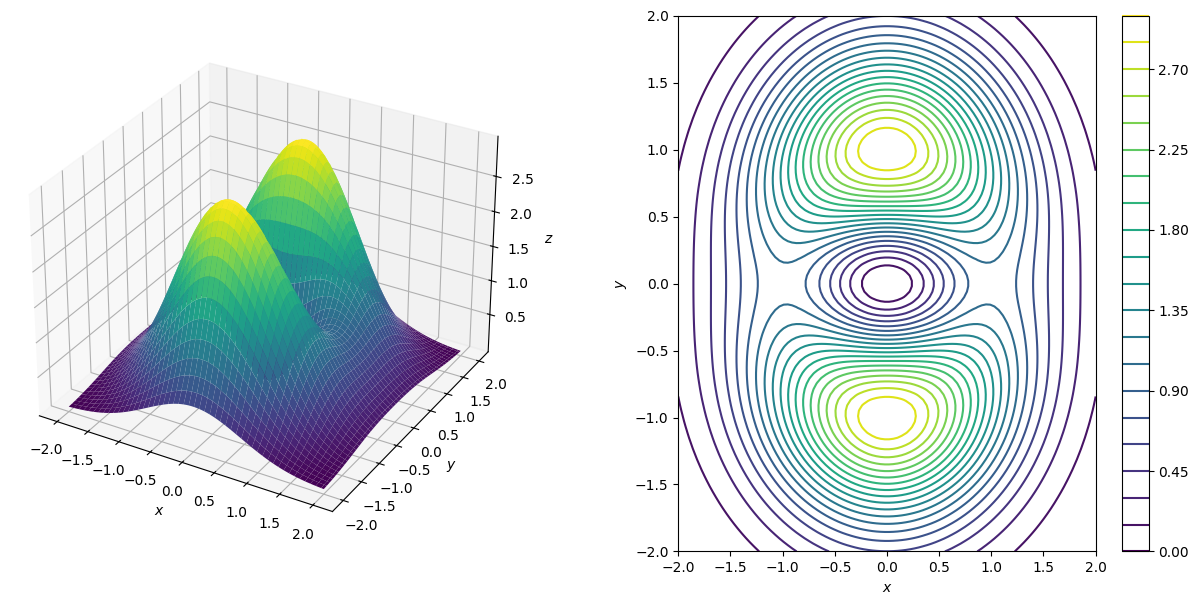
\includegraphics[width=\linewidth]{img/graf1.png}
    \caption{ Gráfica y curvas de nivel de $z=(x^3+3y^2)e^{1-x^2-y^2}$ }
\end{figure}
Para motivar el estudio de funciones de dos variables con valores en $\RR^3$ (caso $n=2$, $m=3$) se puede considerar la representación paramétrica de una ``superficie''. Si $\f(u,v)=(f_1(u,v), f_2(u,v), f_3(u,v))$, se dice que
$$x=f_1(u,v), \quad y=f_2(u,v), \quad z=f_3(u,v)$$
son las ecuaciones paramétricas de una ``superfice'' en el espacio ordinario. Cuando $(u,v)$ recorre el dominio $\Omega\subset\RR^2$ la imagen $\f(u,v)$ recorre una ``superfice'' $S=\f(\Omega)$ que se puede visualizar trazando en el espacio $(x,y,z)$ las ``curvas'' imágenes de las rectas $u=cte$, $v=cte$. Obsérvese que toda ``superficie'' dada en forma explícita $z=f(x,y)$ admite una parametrización canónica $\f(u,v)=(u,v,f(u,v))$.

Un ejemplo estandar lo proporciona la parametrización usual de la esfera de centro $(0,0,0)$ y radio $R$, usando los parámetros habituales, latitud $\varphi$, y longitud $\theta$:
$$x=R\cos\varphi\cos\theta, \quad y=R\cos\varphi\sen\theta, \quad z=R\sen\varphi$$
Según sea el dominio $\Omega$ donde varían los parámetros se obtendrá como imagen un trozo de esfera, o toda la esfera. Así por ejemplo, el trozo de esfera que queda en $\conj{(x,y,z): y>0, \ z>0}$ se parametriza con $\Omega=\conj{(\varphi,\theta): 0<\varphi<\pi/2, \ 0<\theta<\pi}$.

\subsubsection*{Funciones de tres variables}

Una motivación geométrica para el estudio de las funciones reales de tres variables reales es el de las ``superficies'' definidas mediante una ecuación de la forma $g(x,y,z)=c$, como es el caso de la esfera $x^2+y^2+z^2=1$. Estas ``superficies'' se dice que admiten una representación {\it implícita} mediante la ecuación $g(x,y,z)=c$. Es claro que cualquier ``superficie'' dada en forma explícita $z=f(x,y)$ se puede representar implícitamente usando la ecuación $g(x,y,z)=0$ donde $g(x,y,z)=f(x,y)-z$. Con la esfera se pone de manifiesto que la clase de las ``superficies'' que admiten una ecuación implícita es estrictamente más amplia que la clase de las que admiten una representación explícita. (El teorema de la función implícita permitirá estudiar cuando una ``superficie'' dada en forma implícita admite representaciones explícitas locales).

La gráfica de una función real de tres variables reales (caso $n=3$, $m=1$) es un subconjunto de $\RR^4$ y es imposible visualizarla. Una alternativa para visualizar geométricamente la función y dar interpretaciones físicas de su comportamiento es considerar sus ``superficies'' de nivel
$$N_c=\conj{ (x,y,z)\in\Omega : f(x,y,z)=c}$$
Estas ``superficies'', dadas en  forma implícita, se pueden visualizar en el espacio ordinario. Cuando se interpreta que la función $t=f(x,y,z)$ proporciona la temperatura $t$ del punto $(x,y,z)\in\Omega$, entonces las ``superfices'' de nivel se llaman isotermas y su distribución en el espacio permite apreciar como varía la temperatura en el recinto $\Omega\subset\RR^3$.

Una ``curva'' en el espacio tridimensional $\RR^3$ puede venir dada como intersección de dos ``superficies'' expresadas en forma implícita
$$g_1(x,y,z)=0, \quad g_2(x,y,z)=0$$
En el estudio de una curva de esta clase interviene una función de tres variables reales con valores en $\RR^2$, $\g(x,y,z)=(g_1(x,y,z), g_2(x,y,z))$. El teorema de la función implícita servirá para decidir cuando una ``curva'' de este tipo admite una representación paramétrica local.

\section{Coordenadas curvilíneas}

En el caso $n=2$ y $m=2$, una función $\f(u,v)=(f_1(u,v),f_2(u,v))$ se puede interpretar como una transformación entre dos planos: El plano $(u,v)$ donde varían las variables independientes y el plano $(x,y)$ donde toman valores las variables dependientes $x=f_1(u,v)$, $y=f_2(u,v)$. La transformación se puede visualizar considerando las curvas, en el plano $(x,y)$, imágenes de las rectas $u=cte$, $v=cte$. Estas transformaciones intervienen en los problemas de cambio de variable en cálculo diferencial e integral. En este asunto, un problema expresado en términos de las variables originales $(x,y)$ mediante la sustitución $x=f_1(u,v)$, $y=f_2(u,v)$ se transforma en otro problema en términos de las nuevas variables $(u,v)$.

Un ejemplo notable lo proporciona el cambio de variable a {\it coordenadas polares}, asociado a la transformación
$$\g(r,\theta)=(r\cos\theta, r\sen\theta)$$

En este caso, si $(x,y)=(r\cos\theta, r\sen\theta)$, con $r\geq 0$, se dice que $(r,\theta)$ son las coordenadas polares del punto $(x,y)$. Las coordenadas polares de un punto $(x,y)\neq (0,0)$ son únicas cuando se exige que $\theta$ varíe en un intervalo $(\alpha,\beta)$ con $\beta - \alpha\leq 2\pi$.

En el caso $n=3$, $m=3$, una función $\f(t,u,v)=(f_1(t,u,v),f_2(t,u,v),f_3(t,u,v))$ se puede interpretar como una transformación en el espacio $\RR^3$. En una copia del espacio varían las variables independientes $(t,u,v)$ y en la otra toman valores las variables dependientes, $x=f_1(t,u,v)$, $y=f_2(t,u,v)$, $z=f_3(t,u,v)$. Igual que en el caso $n=2$, $m=2$ estas transformaciones intervendrán en los problemas de cambio de variable, donde un problema expresado en términos de las variables originales $(x,y,z)$ mediante la sustitución $x=f_1(t,u,v)$, $y=f_2(t,u,v)$, $z=f_3(t,u,v)$ se transforma en otro problema en términos de las nuevas variables $(t,u,v)$.

Un ejemplo importante es el cambio de variable a {\it coordenadas esféricas}. Estas coordenadas son las asociadas a la transformación
$$\g(\rho,\varphi,\theta)=(\rho\cos\varphi\cos\theta,\rho\cos\varphi\sen\theta, \rho\sen\varphi)$$
En este caso, si $(x,y,z)=(\rho\cos\varphi\cos\theta,\rho\cos\varphi\sen\theta, \rho\sen\varphi)$ con $\rho\geq 0$, se dice que $(\rho,\varphi,\theta)$ son las coordenadas esféricas del punto $(x,y,z)$, a las variables $\varphi$, $\theta$ se les llama latitud y longitud por su interpretación obvia como coordenadas geográficas. Las coordenadas esféricas de un punto $(x,y,z)$, con $(x,y)\neq (0,0)$, son únicas cuando se exige que $\theta$ varíe en un intervalo $(\theta_0,\theta_1)$ con $\theta_1-\theta_0\leq 2\pi$ y que $\varphi$ varíe en un intervalo $(\varphi_0,\varphi_1)\subset(-\pi/2, \pi/2)$.

Otro ejemplo notable lo proporcionan las {\it coordenadas cilíndricas}, asociadas a la transformación
$$\g(r,\theta, t)=(r\cos\theta,r\sen\theta,t)$$
Si $(x,y,z)=(r\cos\theta,r\sen\theta,t)$ con $r\geq 0$, se dice que $(r,\theta,t)$ son las coordenadas cilíndricas del punto $(x,y,z)$. Si $(x,y)\neq (0,0)$ las coordenadas cilíndricas de $(x,y,z)$ son únicas cuando se exige que $\theta$ varíe en un intervalo $(\theta_0,\theta_1)$ con $\theta_1-\theta_0\leq 2\pi$.

Cierto tipo de conjuntos $M\subset\RR^3$ se describen fácilmente usando coordenadas esféricas o cilíndricas. Como esta descripción se utilizará con frecuencia al efectuar cambios de variable en integrales triples, conviene adquirir destreza en el problema geométrico de describir subconjuntos de $\RR^3$ usando este tipo de coordenadas.

\section{Ejercicios propuestos}

\begin{ejer}
    Sea $\f(t)=(f_1(t),\dots,f_n(t))$, $t\in [a,b]$ una trayectoria de clase $C^1$, que describe la curva $C=\f([a,b])$ y cumple la condición
    $$(f'_1(t),\dots,f'_n(t))\neq (0,\dots,0)\text{ para cada }t\in [a,b]$$
    Demuestre que la trayectoria sólo pasa un número finito de veces por cada punto de la curva $C$.
\end{ejer}

\begin{reader}
    \begin{proof}[Solución] Supongamos que existe un punto $\p$ en la trayectoria por el que la curva pasa infinitas veces. Sea $\conj{t_n}_{n=1}^\infty$ una sucesión infinita, tal que $\f(t_n)=\p$ para todo $n\in\NN$. Puesto que la sucesión está contenida en el compacto $[a,b]$, por el teorema de Bolzano-Weierstrass, debe tener un punto de acumulación $s$. Sea $\conj{t_{n_k}}_{k=1}^\infty$ una subsucesión de $\conj{t_n}_{n=1}^\infty$ que converja a $s$. 
    
    Fijemos $i\in\conj{1,\dots,n}$ y apliquemos el teorema del valor medio a la función $f_i$ para obtener $s_{k,i} \in[t_{n_k},t_{n_{k+1}}]$ tal que $f'_i(s_{k,i})=0$ para cada $k\in\NN$. Como la sucesión $\conj{s_{k,i}}_{k=1}^\infty$ converge a $s$ y $f'_i$ es continua, se tiene que $f'_i(s)=0$. Como esto es cierto para cada $i\in\conj{1,\dots,n}$, resulta que $\f'(s)=0$ llegando a una contradicción. Por lo que la trayectoria solo pasa un número finito de veces por cada punto de $C$.
    \end{proof}
\end{reader}